% This file was created by tikzplotlib v0.8.5.
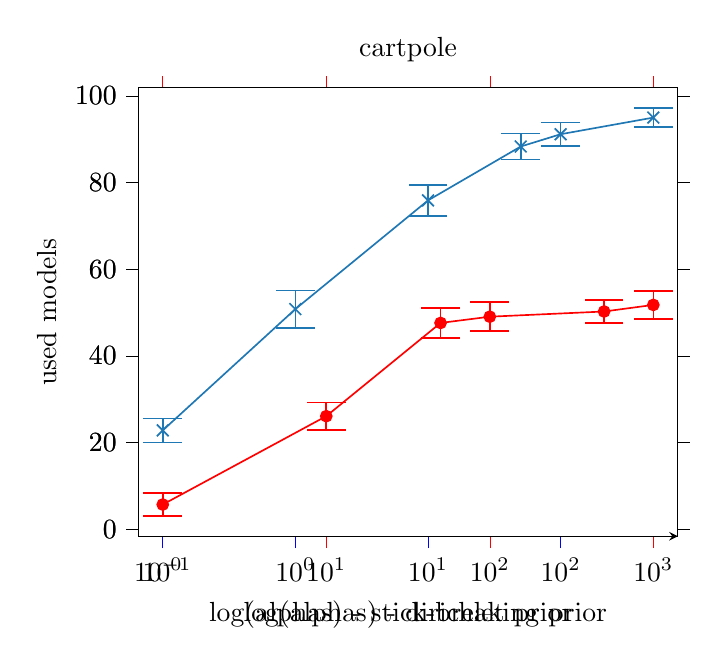
\begin{tikzpicture}

\definecolor{color0}{rgb}{0.12156862745098,0.466666666666667,0.705882352941177}

\begin{axis}[
log basis x={10},
tick align=outside,
tick pos=both,
title={cartpole},
x grid style={white!69.01960784313725!black},
xlabel={log(alphas) - stick-breaking prior},
xmin=0.707945784384138, xmax=1412.53754462275,
xmode=log,
xtick style={color=red},
xtick={0.01,0.1,1,10,100,1000,10000,100000},
xticklabels={\(\displaystyle {10^{-2}}\),\(\displaystyle {10^{-1}}\),\(\displaystyle {10^{0}}\),\(\displaystyle {10^{1}}\),\(\displaystyle {10^{2}}\),\(\displaystyle {10^{3}}\),\(\displaystyle {10^{4}}\),\(\displaystyle {10^{5}}\)},
y grid style={white!69.01960784313725!black},
ylabel={used models},
ymin=-1.62725483214855, ymax=101.857938339759,
ytick style={color=black}
]
\path [draw=red, semithick]
(axis cs:1,3.07661758475632)
--(axis cs:1,8.28338241524368);

\path [draw=red, semithick]
(axis cs:10,22.9061064920196)
--(axis cs:10,29.2538935079804);

\path [draw=red, semithick]
(axis cs:50,44.1358983848622)
--(axis cs:50,51.0641016151378);

\path [draw=red, semithick]
(axis cs:100,45.6995808646219)
--(axis cs:100,52.3804191353781);

\path [draw=red, semithick]
(axis cs:500,47.6588374712157)
--(axis cs:500,52.8211625287843);

\path [draw=red, semithick]
(axis cs:1000,48.4824399319006)
--(axis cs:1000,55.0375600680994);

\addplot [semithick, red, mark=-, mark size=7, mark options={solid}, only marks]
table {%
1 3.07661758475632
10 22.9061064920196
50 44.1358983848622
100 45.6995808646219
500 47.6588374712157
1000 48.4824399319006
};
\addplot [semithick, red, mark=-, mark size=7, mark options={solid}, only marks]
table {%
1 8.28338241524368
10 29.2538935079804
50 51.0641016151378
100 52.3804191353781
500 52.8211625287843
1000 55.0375600680994
};
\addplot [semithick, red, mark=*, mark size=2, mark options={solid}]
table {%
1 5.68
10 26.08
50 47.6
100 49.04
500 50.24
1000 51.76
};
\end{axis}

\begin{axis}[
axis x line=top,
log basis x={10},
tick align=outside,
tick pos=both,
x grid style={white!69.01960784313725!black},
xlabel={log(alphas) - dirichlet prior},
xmin=0.0653208007180445, xmax=765.452956031932,
xmode=log,
xtick style={color=blue},
xtick={0.001,0.01,0.1,1,10,100,1000,10000},
xticklabels={\(\displaystyle {10^{-3}}\),\(\displaystyle {10^{-2}}\),\(\displaystyle {10^{-1}}\),\(\displaystyle {10^{0}}\),\(\displaystyle {10^{1}}\),\(\displaystyle {10^{2}}\),\(\displaystyle {10^{3}}\),\(\displaystyle {10^{4}}\)},
y grid style={white!69.01960784313725!black},
ymin=-1.62725483214855, ymax=101.857938339759,
ytick style={color=black}
]
\path [draw=color0, semithick]
(axis cs:0.1,20.0287187078898)
--(axis cs:0.1,25.5712812921102);

\path [draw=color0, semithick]
(axis cs:1,46.4825933710154)
--(axis cs:1,55.1174066289846);

\path [draw=color0, semithick]
(axis cs:10,72.3436742231519)
--(axis cs:10,79.4163257768481);

\path [draw=color0, semithick]
(axis cs:50,85.3170680993402)
--(axis cs:50,91.3229319006598);

\path [draw=color0, semithick]
(axis cs:100,88.422409818837)
--(axis cs:100,93.897590181163);

\path [draw=color0, semithick]
(axis cs:500,92.8459340771462)
--(axis cs:500,97.1540659228538);

\addplot [semithick, color0, mark=-, mark size=7, mark options={solid}, only marks]
table {%
0.1 20.0287187078898
1 46.4825933710154
10 72.3436742231519
50 85.3170680993402
100 88.422409818837
500 92.8459340771462
};
\addplot [semithick, color0, mark=-, mark size=7, mark options={solid}, only marks]
table {%
0.1 25.5712812921102
1 55.1174066289846
10 79.4163257768481
50 91.3229319006598
100 93.897590181163
500 97.1540659228538
};
\addplot [semithick, color0, mark=x, mark size=3, mark options={solid}]
table {%
0.1 22.8
1 50.8
10 75.88
50 88.32
100 91.16
500 95
};
\end{axis}

\end{tikzpicture}
